\documentclass[final]{beamer}
\usepackage[ngerman]{babel}
\usepackage[utf8]{inputenc}
\usepackage[T1]{fontenc}
\usepackage{csquotes}
\usepackage{eurosym}
\usepackage{lmodern}
\usepackage{listings}
\usepackage{graphicx}
\usepackage{color}
\usepackage{amssymb}

\newcommand{\ThemeFolder}{FSIBeamerTheme}
\RequirePackage{\ThemeFolder/beamerthemeFSI}


\DeclareGraphicsExtensions{.pdf,.png}

\mode<presentation>

\title{Programmiervorkurs für Erstsemester}

\setbeamertemplate{title page}{
  \begin{center}
    \color{FSIblue}
      \resizebox{\textwidth}{!}{Programmiervorkurs}\\
      \vspace{0.3\baselineskip}
      \huge{Einführung in Java}\\
      \huge{Tag 4}
      \vfill
      \large{Tobias Kerst}\\
      \tiny{SS 2015}
  \end{center}
}

\begin{document}

\lstset{
	breakatwhitespace=true,
	breaklines=true,
	extendedchars=true,
	inputencoding=utf8,
	language=java,
	literate={€}{{\euro}}1 {ä}{{\"a}}1 {ö}{{\"o}}1 {ü}{{\"u}}1,
	numbers=none,
	numbersep=5pt,
	numberstyle=\tiny,
	showstringspaces=true,
	tabsize=3,
%	backgroundcolor=\color{lightgray},
	basicstyle=\color{black}\small\ttfamily,
	commentstyle=\color{gray},
	identifierstyle=\color{cyan},
	keywordstyle=\color{orange},
	stringstyle=\color{purple}
}

\begin{frame}
  \titlepage
\end{frame}

\begin{frame}
	\frametitle{Inhaltsübersicht Vorkurs}
	\begin{itemize}
	{\color{gray}
		\item {Tag 1: Variablen, Datentypen, Konvertierungen, Arithmetik, Netbeans, Einführung Debugging}
		\item {Tag 2: Boolesche Ausdrücke, Kommentare, If-Abfragen, Switch-Case, Weiterführung Debugging}
		\item {Tag 3: Arrays, (Do-)While-Schleife, For-Schleifen, Weiterführung Debugging}
		{\color{black}
		\item {Tag 4: (statische) Methoden, Klassenvariablen, JavaDoc, Exceptions}
		}
	}
	\end{itemize}
\end{frame}

\section{Ablauf}
\begin{frame}
  \frametitle{Ablauf}
  \begin{itemize}
    \item{09:30 Vorstellung der Lösungen des Vortages}
    \item{ab 10:00 Vorlesung}
    \item{90 min Mittagspause}
    \item{gegen 12:30 / 13:00 Übungen}
  \end{itemize}
\end{frame}

\section{Methoden}
\begin{frame}[containsverbatim]
	\frametitle{Beispiel ohne Methoden}
	\begin{lstlisting}
public class Main {
	public static void main() {
		for (int i = 1; i <= 10; i++) {
			System.out.println(i);
		}
		
		// weiterer Code
		
		for (int i = 1; i <= 10; i++) {
			System.out.println(i);
		}
	}
}
	\end{lstlisting}
\end{frame}

\subsection{Warum?}
\begin{frame}
	\frametitle{Warum ist der Code problematisch?}
	\textbf{Probleme:}
	\begin{itemize}
		\item{zeitaufwändig}
		\item{(zu) viel Code}
		\item{unübersichtlich}
		\item{Änderungen kosten noch mehr Zeit}
		\item{Code oft nicht wiederverwendbar}
		\item{Arbeitsteilung kaum möglich}
	\end{itemize}
	\pause
	\vspace{\baselineskip}
	\textbf{Lösungen?}
	\pause
	\begin{itemize}
		\item{ähnlichen Code auslagern}
		\item{wiederverwendbaren Code schreiben}
		\item{\textbf{Methoden!}}
	\end{itemize}
\end{frame}

\begin{frame}[containsverbatim]
	\frametitle{Beispiel mit Methoden}
	\begin{lstlisting}
public class Main {
	public static void main () {
		zaehlBisZehn();
		
		// weiterer Code
		
		zaehlBisZehn();
	}
	
	public static void zaehlBisZehn() {
		for (int i = 1; i <= 10; i++) {
			System.out.println(i);
		}
	}
}
	\end{lstlisting}
\end{frame}

\subsection{Wie?}
\begin{frame}[containsverbatim]
	\frametitle{Kopf der Methode}
	\begin{lstlisting}
public static void zaehlBisZehn () { 
	...
}
	\end{lstlisting}
	\begin{itemize}
		\item{\textbf{public static} immer am Anfang (wird im Vorkurs nicht behandelt)}
		\item{\textbf{Rückgabetyp} was gibt mir die Methode zurück}
		\item{\textbf{Methodenname} vor den runden Klammern}
	\end{itemize}
\end{frame}

\subsection{Mehr!}
\begin{frame}
	\frametitle{Methoden können mehr!}
	\begin{itemize}
		\item{Beim Methodenaufruf können zusätzliche Informationen (= Parameter) an die Methode übergeben werden}
		\item{Methoden können Informationen an den Aufrufer zurück geben}
		\item{Methoden können sich selbst aufrufen (= Rekursion) (nicht Teil des Vorkurses)}
	\end{itemize}
\end{frame}

\begin{frame}[containsverbatim]
	\frametitle{Aufruf einer Methode}
	\begin{lstlisting}
	public static void main() {
		zaehlBisZehn();
		int x = gibMir42();
		int y = verdoppelWert(x);
	\end{lstlisting}
	\begin{itemize}
		\item{Methodenname}
		\item{(Parameter)}
		\item{;}
	\end{itemize}
\end{frame}

\subsubsection{Methoden mit Parameter}
\begin{frame}[containsverbatim]
	\frametitle{Beispiel ohne Methoden}
	\begin{lstlisting}[escapechar=!]
public class Main () {
	public static void main() {
		for (int i = 1; i <= !\color{red}\textbf{9}!; i++) {
			System.out.println(i);
		}
		
		// weiterer Code
		
		for (int i = 1; i <= !\color{red}\textbf{10}!; i++) {
			System.out.println(i);
		}
	}
}
	\end{lstlisting}
\end{frame}

\begin{frame}[containsverbatim]
	\frametitle{Beispiel mit Methoden}
	\begin{lstlisting}[escapechar=!]
public class Main() {
	public static void main() {
		zaehleBis(!\color{red}\textbf{9}!);
		
		// weiterer Code
		
		zaehleBis(!\color{red}\textbf{10}!);
	}

	public static void zaehleBis(!\textbf{\color{blue}int \color{red}z}!) {
		for (int i = 1; i <= !\color{red}\textbf{z}!; i++) {
			System.out.println(i);
		}
	}
}
	\end{lstlisting}
\end{frame}

\begin{frame}[containsverbatim]
	\frametitle{Kopf der Methode}
	\begin{lstlisting}[escapechar=!]
public static void zaehleBis(!\color{blue}int \color{red}z!) {
	...
}
	\end{lstlisting}
	\begin{itemize}
		\item{In die runden Klammern kommen die Paramter}
		\item{Parameter werden mit Komma getrennt:
			\begin{lstlisting}[escapechar=!]
(!\color{blue}int \color{red}a!, !\color{blue}boolean \color{red}b!, !\color{blue}double \color{red}c!)
			\end{lstlisting}
		}
		\item{Ein Parameter besteht aus {\color{blue}Datentyp} und \color{red}Bezeichner}
	\end{itemize}
\end{frame}

\begin{frame}[containsverbatim]
	\frametitle{Aufruf}
	\begin{lstlisting}[escapechar=!]
pulic static void main() {
	zaehleBis(!\color{red}9!);
	zaehleBis(!\color{red}10!);
}
	\end{lstlisting}
	\begin{itemize}
		\item{Parameter, die man übergeben möchte, durch Komma getrennt in die Runden Klammern}
	\end{itemize}
\end{frame}

\begin{frame}[containsverbatim]
	\frametitle{Was passiert?}
	\begin{itemize}
		\item{
			\begin{lstlisting}[escapechar=!]
zaehleBis(!\color{red}9!);
			!\vspace{\baselineskip}!
public static void zaehleBis(!\color{blue}int \color{red}z!) {
	// z wird der Wert 9 zugewiesen
}
			\end{lstlisting}
		}
		\vspace{\baselineskip}
		\item{
			\begin{lstlisting}[escapechar=!]
zaehleBis(!\color{red}10!);
			!\vspace{\baselineskip}!
public static void zaehleBis(!\color{blue}int \color{red}z!) {
	// z wird der Wert 10 zugewiesen
}
			\end{lstlisting}
		}
	\end{itemize}
\end{frame}

\begin{frame}[containsverbatim]
	\frametitle{Beispiel mit 2 Parametern}
	\begin{lstlisting}[escapechar=!]
public class Main {
	public static void main() {
		zaehleVonBis(!\color{blue}1!, !\color{red}9!);
		// weiterer Code
		zaehleVonBis(!\color{blue}5!, !\color{red}10!);
	}
	
	public static void 
		zaehleVonBis(int !\color{blue}v!, int !\color{red}b!) {
		for (int i = !\color{blue}v!; i <= !\color{red}b!; i++) {
			System.out.println(i);
		}
	}
}
	\end{lstlisting}
\end{frame}

\subsubsection{Methoden mit Rückgabewert}
\begin{frame}[containsverbatim]
	\frametitle{Beispiel mit Rückgabewert}
	\begin{lstlisting}[escapechar=!]
public class Main {
	public static void main() {
		!\color{blue}int! !\color{red}x! = zaehleVonBis(1, 9);
	}
	
	public static !\color{blue}int! 
		zaehleVonBis(int v, int b) {
		for (int i = v; i <= b; i++) {
			System.out.println(i);
		}
		
		!\color{blue}return! !\color{red}b - v + 1!;
	}
}
	\end{lstlisting}
\end{frame}

\begin{frame}[containsverbatim]
	\frametitle{Kopf der Methode}
	\begin{lstlisting}[escapechar=!]
public static !\color{blue}int! zaehleVonBis(int v, int b) {
	...
	!\color{blue}return! !\color{red}b - v + 1!;
}
	\end{lstlisting}
	\begin{itemize}
		\item{Möchte man keinen Wert zurück geben, so kommt nach \textbf{static} das Schlüsselwort \color{blue}void}
		\item{Ansonsten wird {\color{blue}void} durch den gewünschten Datentyp ersetzt}
		\item{Mit {\color{blue}return} wird der Wert zurückgegeben. Das {\color{blue}return} ist Pflicht und muss erreicht werden}
	\end{itemize}
\end{frame}

\begin{frame}[containsverbatim]
	\frametitle{Was passiert?}
	\begin{lstlisting}[escapechar=!]
!\color{blue}int! !\color{red}x! = zaehleVonBis(1, 9);
	\end{lstlisting}
	\begin{itemize}
		\item{Rechte Seite von "\textbf{=}"\ wird zuerst ausgewertet
			\begin{itemize}
				\item{zaehleVonBis(1, 9);}
			\end{itemize}
		}
	\end{itemize}
	\begin{lstlisting}[escapechar=!]
public static !\color{blue}int! zaehleVonBis(int v, int b) {
	...
	!\color{blue}return! !\color{red}b - v + 1!;
}
	\end{lstlisting}
	\begin{itemize}
		\item{v = 1, b = 9
			\begin{itemize}
				\item{return 9 - 1 + 1 = 9}
					\begin{itemize}
						\item{9 wird zurückgegeben}
					\end{itemize}
			\end{itemize}
		}
		\item{{\color{red}x} wird der Wert 9 zugewiesen}
	\end{itemize}
\end{frame}

\begin{frame}[containsverbatim]
	\frametitle{Generell}
	\begin{lstlisting}[escapechar=!]
public static !\color{orange}Rückgabetyp! !\color{black}Name! (!\color{red}Parameter!) {
	// Methodenrumpf
	!\color{blue}return! ... ; 
}
	\end{lstlisting}
	\begin{itemize}
		\item{Wenn der {\color{blue}Rückgabetyp} \textbf{void} ist, darf das {\color{blue}return} keinen Rückgabewert haben und ist optional}
	\end{itemize}
\end{frame}

\subsubsection{Beispiel Lesbarkeit}

\begin{frame}[containsverbatim]
	\frametitle{Lesbarkeit durch Methoden}
	\begin{itemize}
	\item{Berechnung der Fakultät: $n! = 1 \times 2 \times \dots \times n$}
	\end{itemize}
	\begin{lstlisting}[escapechar=!]
	static long fak(int n)
    {
        long faku = 1;
        // Iterative Berechnung
        for(int i = 1; i<=n; i++)
        {
            faku *= i;
        }
        return faku;
    } 
	\end{lstlisting}
	\begin{itemize}
		\item{Um Fakultät zu berechnen benötigt man eine Schleife}
	\end{itemize}
\end{frame}

\begin{frame}[fragile]
	\frametitle{Binomialkoeffizient berechnen}
	\[\left(\!\!\!
  	\begin{array}{c}
	    n \\
	    k
	\end{array}
	  \!\!\!\right) = \frac{n!}{(n-k)! \times k!}
	\]
	\begin{itemize}
		\item{Für die Berechnung braucht man 3 Mal eine Fakultät}
		\item{Somit 3 Schleifen in der Berechnung}
		\item{Code unlesbar}
	\end{itemize}
	\pause
	\textbf{Lösung}
	\begin{itemize}
		\item{Methode \texttt{long fak(int n)} benutzen}
	\end{itemize}
	\pause
	\begin{lstlisting}[basicstyle=\tiny]
	static double berechneBinomialkoeffizient(int n, int k) {
	    double bin = fak(n) / (fak(n - k) * fak(k));
	    return bin;
	}
	\end{lstlisting}
\end{frame}

\section{Klassenvariablen}
\begin{frame}[containsverbatim]
	\frametitle{Beispiel ohne Klassenvariablen}
	\begin{lstlisting}[escapechar=!]
public class Main {
	public static void main() {
		!\color{blue}int! !\color{red}x! = zaehleVonBis(1, 9);
	}
	
	public static !\color{blue}int! 
		zaehleVonBis(int v, int b) {
		for (int i = v; i <= b; i++) {
			System.out.println(i);
		}
		
		boolean wurdeAusgegeben = b >= v;
		
		!\color{blue}return! !\color{red}b - v + 1!;
	}
}
	\end{lstlisting}
\end{frame}

\subsection{Warum?}
\begin{frame}
	\frametitle{Warum?}
	\textbf{Probleme}
	\begin{itemize}
		\item{Methoden können nur einen Wert zurückgeben}
		\item{Eine Methode kann nicht auf Daten aus anderen Methoden zugreifen}
	\end{itemize}
	\vspace{\baselineskip}
	\pause
	\textbf{Lösungen}
	\pause
	\begin{itemize}
		\item{\textbf{Klassenvariablen}
			\begin{itemize}
				\item{mit Bedacht verwenden!}
			\end{itemize}
		}
	\end{itemize}
\end{frame}
	
\subsection{Wie?}
\begin{frame}[containsverbatim]
	\frametitle{Beispiel mit Klassenvariablen}
	\begin{lstlisting}[escapechar=!]
public class Main {
	!\color{blue}public static boolean! !\color{red}wurdeAusgegeben!;
	public static void main() {
		int x = zaehleVonBis(1, 9);
		System.out.println(wurdeAusgegeben);
	}
	
	public static int 
		zaehleVonBis(int v, int b) {
		for (int i = v; i <= b; i++) {
			System.out.println(i);
		}
		!!\color{red}wurdeAusgegeben! = b >= v;
		return b - v + 1;
	}
}
	\end{lstlisting}
\end{frame}

\begin{frame}[containsverbatim]
	\frametitle{Deklaration von Klassenvariablen}
	\begin{itemize}
		\item{Deklaration direkt nach Klassendeklaration}
		\item{\textbf{public static} {\color{blue}Datentyp} {\color{red}Variablenname};}
		\item{sichtbar in der ganzen Klasse}
		\item{Ohne manuelle Zuweisung wird der Defaultwert zugewiesen}
		\item{Beispiel:
			\begin{lstlisting}[escapechar=!]
public static !\color{blue}boolean! !\color{red}wurdeAusgegeben!;
			\end{lstlisting}
		}
	\end{itemize}
\end{frame}

\section{Aufgabe}
\begin{frame}
	\frametitle{Vorstellung der Aufgabe}
	\begin{columns}[T]
		\column{0.5\textwidth}
			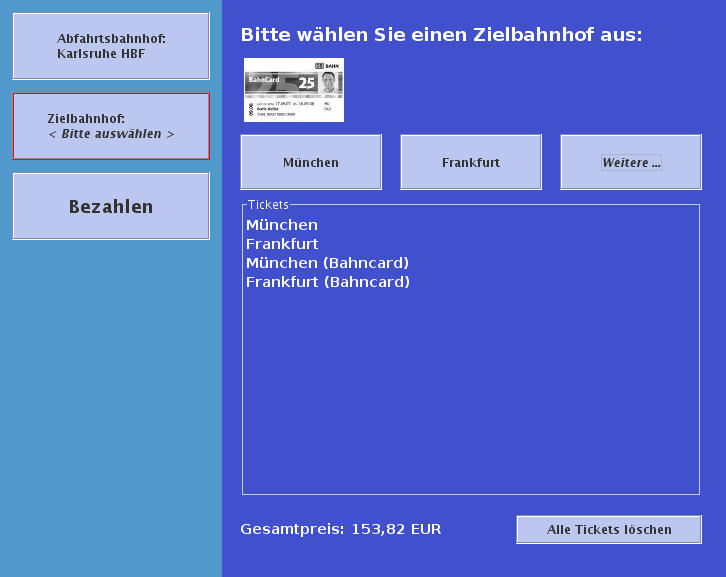
\includegraphics[width=\textwidth]{gfx/bahnticketautomat_buchen}
		\column{0.5\textwidth}
			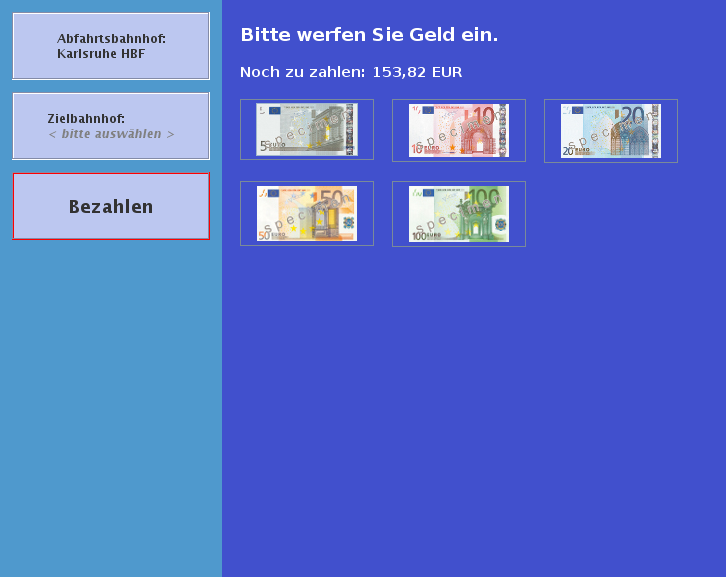
\includegraphics[width=\textwidth]{gfx/bahnticketautomat_bezahlen}
	\end{columns}
	\vspace{\baselineskip}
	\begin{columns}[T]
		\column{0.5\textwidth}
			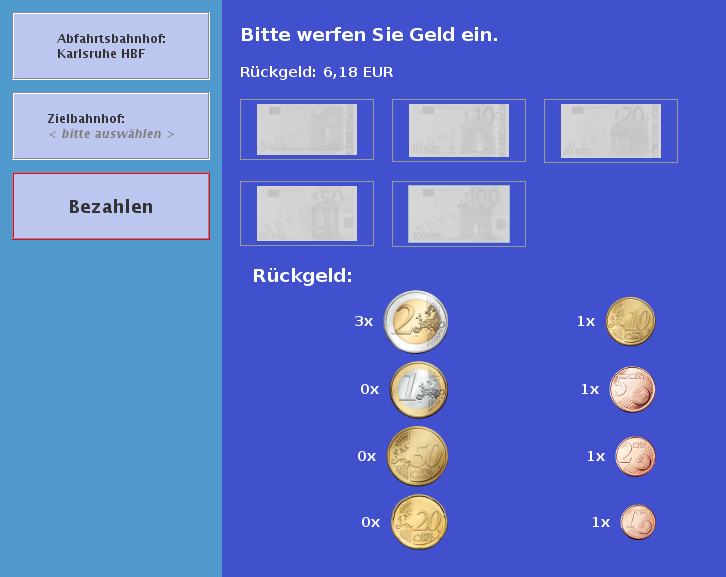
\includegraphics[width=\textwidth]{gfx/bahnticketautomat_rueckgeld}
		\column{0.5\textwidth}
		\pause
			
\includegraphics[width=\textwidth]{gfx/Wait-what-meme-rage-face.jpg}
	\end{columns}
\end{frame}

\subsection{Methoden}
\begin{frame}
	\frametitle{Methoden}
	\begin{itemize}
		\item{{\color{blue}public static} String[] \textbf{addNewTicket}(String[] oldTickets, String newTicket, {\color{blue}boolean} bahncard)}
		\item{{\color{blue}public static void} \textbf{calculateNewSum}({\color{blue}int} distance, {\color{blue}boolean} bahncard)}
		\item{{\color{blue}public static double} \textbf{getSum}()}
		\item{{\color{blue}public static void} \textbf{resetSum}()}
		\item{{\color{blue}public static void} \textbf{beginPayment}()}
		\item{{\color{blue}public static void} \textbf{insertMoney}({\color{blue}int} amount)}
		\item{{\color{blue}public static double} \textbf{getAmountLeft}()}
		\item{{\color{blue}public static boolean} \textbf{isAmountLeft}()}
		\item{{\color{blue}public static double} \textbf{getChangeAmount}()}
		\item{{\color{blue}public static int}[] \textbf{getChangeCoins}()}
	\end{itemize}
\end{frame}

\subsubsection{addNewTicket}
\begin{frame}
	\frametitle{addNewTicket}
	\begin{itemize}
		\item{Parameter:}
			\begin{itemize}
				\item{oldTickets: String Array enthält die alten Tickets}
				\item{newTicket: String}
				\item{bahncard: boolean}
			\end{itemize}
		\item{Beschreibung:}\\
Soll den Parameter \textbf{\textit{oldTickets}} um den Parameter \textbf{\textit{newTicket}} erweitern und für den fall das der Parameter \textbf{\textit{bahncard}} {\color{blue}true} ist um \enquote{(Bahncard)} erweitern und anschließend zurück geben.
	\end{itemize}
\end{frame}

\subsubsection{getSum}
\begin{frame}
	\frametitle{getSum}
	\begin{itemize}
		\item{Hat keine Parameter}
		\item{Gibt den aktuellen Gesamtpreis als double in Euro zurück}
	\end{itemize}
\end{frame}

\subsubsection{calculateNewSum}
\begin{frame}
	\frametitle{calculateNewSum}
	\begin{itemize}
		\item{Parameter:}
			\begin{itemize}
				\item{distance: integer}
				\item{bahncard: boolean}
			\end{itemize}
		\item{Beschreibung:}
Berechnet den Gesamtpreis aller bisher sowei dem aktuell ausgewählten Ticket. \\
Dabei gilt:\\
			\begin{itemize}
				\item{Bis 200km: 10 \euro + 0.20 \euro pro km}
				\item{Ab 200km: 5 \euro + 0.15 \euro pro km}
				\item{Mit einer Bahncard erhält man immer 25\% Rabatt}
			\end{itemize}
		\item{Hat keinen Rückgabewert}
	\end{itemize}
\end{frame}

\subsubsection{resetSum}
\begin{frame}
	\frametitle{resetSum}
	\begin{itemize}
		\item{Hat keine Parameter}
		\item{Hat keine Rückgabewert}
		\item{Setzt den Gesamtpreis auf 0 zurück}
	\end{itemize}
\end{frame}

\subsubsection{insertMoney}
\begin{frame}
	\frametitle{insertMoney}
	\begin{itemize}
		\item{Parameter:}
			\begin{itemize}
				\item{amount: integer}
			\end{itemize}
		\item{Beschreibung:}
Wenn der Kunde einen Geldschein einwirft wird diese Methode aufgerufen. Der noch noch zu bezahlende Betrag muss dementsprechen angepasst werden
		\item{Hat keinen Rückgabewert}
	\end{itemize}
\end{frame}

\subsubsection{getAmountLeft}
\begin{frame}
	\frametitle{getAmountLeft}
	\begin{itemize}
		\item{Hat keine Parameter}
		\item{Als Rückgabewert soll hier der noch zu zahlende Betrag als double in Euro zurück gegben werden}
	\end{itemize}
\end{frame}

\subsubsection{getChangeAmount}
\begin{frame}
	\frametitle{getChangeAmount}
	\begin{itemize}
		\item{Hat keine Parameter}
		\item{Wird aufgerufen, wenn der Kunde ausreichend Geld eingeworfen hat}
		\item{Gibt den Betrag des Wechselsgeld zurück (in Euro). Dieser muss Positiv sein}
	\end{itemize}
\end{frame}

\subsubsection{getChangeCoins}
\begin{frame}
	\frametitle{getChangeCoins}
	\begin{itemize}
		\item{Hat keine Parameter}
		\item{Beschreibung:}
Berechnet wieviel Münzen von jeder Sorte der Kunde zurück bekommt.
		\item{Gibt ein Array zurück, das die Anzahl der entsprechenden Münzen enthält}
			\begin{itemize}
				\item{Rückgabe[0]: enthält die Anzahl der 2 \euro-Münzen}
				\item{Rückgabe[1]: enthält die Anzahl der 1 \euro-Münzen}
				\item{...}
				\item{Rückgabe[7]: enthält die anzahl der 1 ct-Münzen}
			\end{itemize}
	\end{itemize}
\end{frame}

\subsubsection{beginPayment}
\begin{frame}
	\frametitle{beginPayment (OPTIONAL)}
	\begin{itemize}
		\item{Diese Methode ist Optional}
		\item{Wird nicht immer benötigt}
		\item{Kann für spezielle aktionen zu begin des Bezahlvorgangs verwendet werden}
	\end{itemize}
\end{frame}

\section{Quellen \& Lizenz}
\begin{frame}
	\frametitle{Quellen und Lizenz}
	\begin{center}
		
\includegraphics[width=250px]{gfx/fsi}
	\end{center}
	\begin{itemize}
		\item{Original von Samuel Zeitvogel}
		\item{Überarbeitet 2012 von Daniel Hoff}
		\item{Überarbeitet 2013 von Tristan Wagner}
		\item{Überarbeitet 2015 von Tobias Kerst}
	\end{itemize}
\end{frame}

\end{document}
